%%%%%%%%%%%%%%%%%%%%%%%%%%%%%%%%%%%%%%%%%%%%%%%%%%%%%%%%%%%%%%%%%%%%%%%%
\section{Experimental Setup}
The 2 sister experiments were carried out in Hall A of Jlab, 

% table of beam parameters
\begin{table}
    \centering
    \begin{tabular}{c | c c }
	\hline
	&   PREX-II & CREX  \\
	\hline
	Target	& \Pb	& \Ca	\\
	Beam Energy ($GeV$) & 0.97 & 2.18  \\
	Beam Current ($\mu A$)	& 70	& 150	\\
	Beam Polarization & 88\%   & 87.1\%   \\
	Scattering angle ($\deg$)   & 5	& 4.51 \\
	$Q^2$ ($GeV^2$)	&   & 0.0297	\\
	\hline
	Charge (C)  &	&   \\
	\hline
    \end{tabular}
\end{table}

%%%%%%%%%%%%%%%%%%%%%%%%%%%%%%%%%%%%%%%%%%%%%%%%
\subsection{Design}
Though weak charge distribution is what we want to measure, it doesn't mean we
know nothing about it. Due to the symmetry between proton and neutron, we would
expect the weak charge (neutron) distribution is similar to the charge (proton)
distribution. Based on this assumption, we will have some models to describe
the neutron distribution and therefore the FFs, from which we can derive the
cross section and their asymmetry.

For symmetric nuclei with equal number of proton and neutron, it is expected 
that their density distributions are similar to each other, which are usually
expressed as a 2-parameter Fermi function:
\begin{equation}
    \rho(r) = \frac{\rho_0}{1 + exp(r-a)/c}
\end{equation}
where a and c denote the half-height radius and diffuseness respectively. 
% Thiel et al J.Phys.G 46 (2019) 9, 093003 

\subsubsection{Sensitivity}

%%%%%%%%%%%%%%%%%%%%%%%%%%%%%%%%%%%%%%%%%%%%%%%%
\subsection{Continuous Electron Beam Accelerator Facility (CEBAF)}
\begin{figure}
    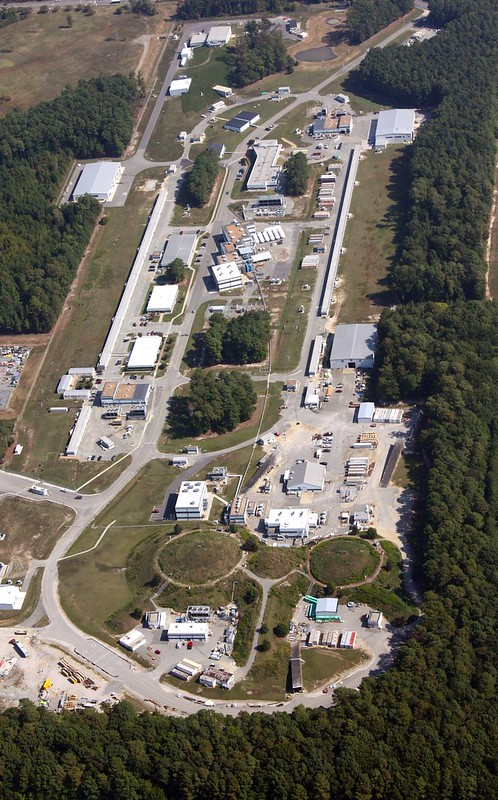
\includegraphics[width=0.44\linewidth]{jlab_1.jpg}
    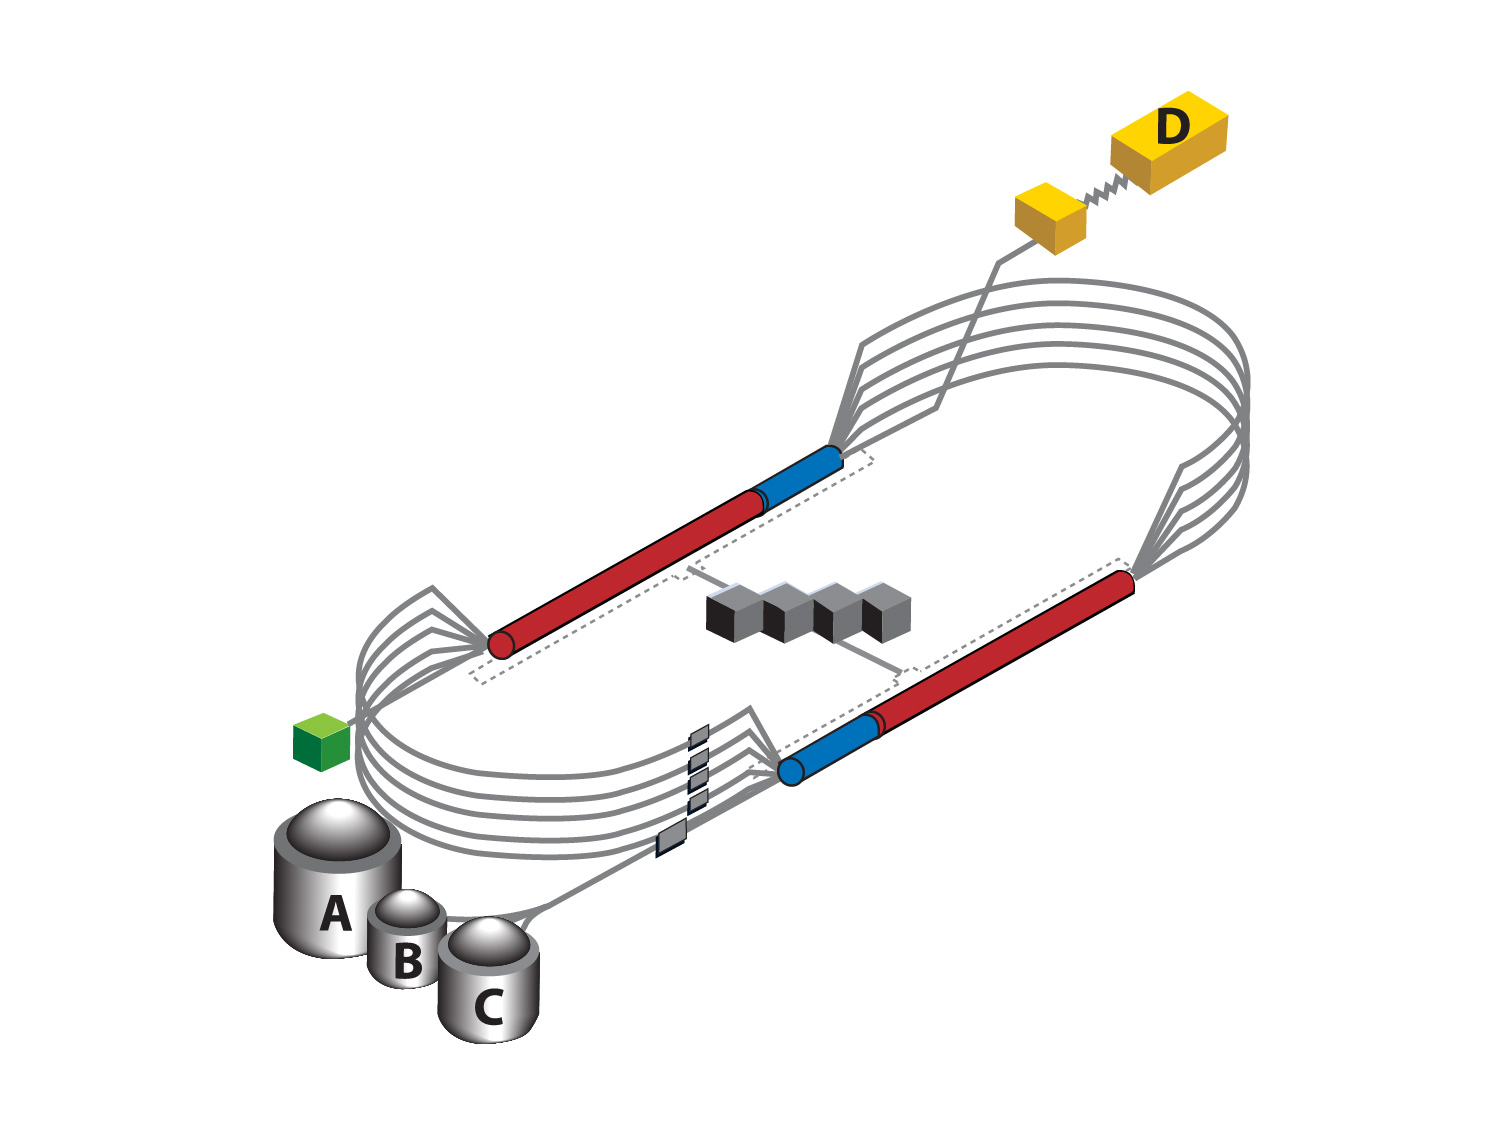
\includegraphics[width=0.8\linewidth]{cebaf}
\end{figure}
With the 12 GeV upgrade, the north and south LINAC each has 25 cryomodules, 
capable of accelrating electrons at the rate of 2.2 $GeV/turn$. The total power
of CEBAF (1 MW) limits the available beam current. For PREX-II (CREX), 
the beam current was 70 (150) $\mu A$ respectively.

%%%%%%%%%%%%%%%%%%%%%%%%%%%%%%%%%%%%%%%%%%%%%%%%
\subsection{Polarized Source}

%%%%%%%%%%%%%%%%%%%%%%%%%%%%%%%%%%%%%%%%%%%%%%%%
\subsection{Polarization Control}

%%%%%%%%%%%%%%%%%%%%%%%%%%%%%%%%%%%%%%%%%%%%%%%%
\subsection{Beam Modulation}

%%%%%%%%%%%%%%%%%%%%%%%%%%%%%%%%%%%%%%%%%%%%%%%%
\subsection{Target}

%%%%%%%%%%%%%%%%%%%%%%%%%%%%%%%%%%%%%%%%%%%%%%%%
\subsection{Magnets}

%%%%%%%%%%%%%%%%%%%%%%%%%%%%%%%%%%%%%%%%%%%%%%%%
\subsection{HRS}

%%%%%%%%%%%%%%%%%%%%%%%%%%%%%%%%%%%%%%%%%%%%%%%%
\subsection{Detector}
